\chapter{Programmation}
\label{chap:programmation}

La plupart des scripts étant conçu pour fonctionner dans AICA Studio et donc \gls{ros2}, il a été nécessaire d'adopter une architecture spécifique pour permettre la communication entre les différents éléments du système. Toutefois, l'objectif du travail n'était pas d'approfondir la compréhension ou la maîtrise de \gls{ros2} en tant que telle.

Ainsi, la plupart des programmes et blocs fonctionnels ont d'abord été développés et testés en Python de façon indépendante, sans intégration directe à AICA Studio. Cette approche a permis de valider les algorithmes et le fonctionnement général dans un environnement plus simple et maîtrisé.

Dans un second temps, quand le développement a été finalisé, l'intégration dans l'environnement AICA Studio a été réalisée. Cette étape a consisté à adapter les scripts pour qu'ils fonctionnent avec l'architecture \gls{ros2} imposée par AICA Studio, en veillant à la compatibilité des communications et à l'intégration des blocs fonctionnels dans le système global.

Cette démarche a permis de gagner du temps sur le développement initial, tout en assurant une intégration robuste et conforme aux exigences de la plateforme finale.

\section{Ecran tactile}
L'écran tactile ED101 est le seul élément de la maquette qui n'est pas directement lié au logiciel AICA Studio. Un script Python a été développé avec la bibliothèque \texttt{tkinter} pour permettre à l'utilisateur de dessiner et d'envoyer directement le fichier DXF correspondant au PC principal. Un Bloc fonctionnel a été créé dans AICA Studio pour recevoir ce fichier DXF.

\begin{figure}[H]
    \centering
    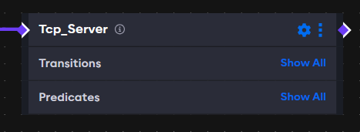
\includegraphics[width=0.8\textwidth]{assets/figures/AICA_Tcp_Server.png}
    \caption{Bloc fonctionnel du serveur TCP dans AICA Studio}
    \label{fig:touchscreen_interface}
\end{figure}

\section{Graveuse laser}
Afin de pouvoir communiquer avec la graveuse laser depuis le logiciel AICA Studio, un bloc fonctionnel a été développé afin de :
\begin{itemize}
    \item Charger un fichier DXF.
    \item Convertir le fichier DXF en G-code.
    \item Envoyer le G-code à la graveuse laser.
    \item Gérer la synchronisation entre le bras robot et la graveuse laser.
\end{itemize}

\begin{figure}[H]
    \centering
    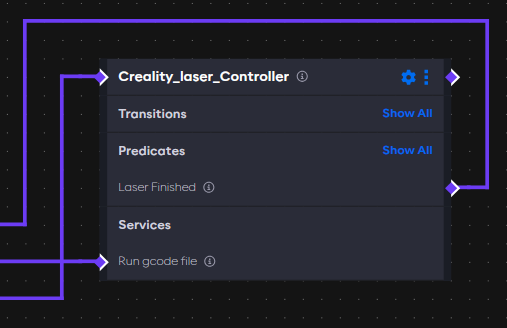
\includegraphics[width=0.8\textwidth]{assets/figures/AICA_Laser_interface.png}
    \caption{Bloc fonctionnel de la graveuse laser dans AICA Studio}
    \label{fig:laser_interface}
\end{figure}

Le bloc fonctionnel offre une certaine liberté dans le choix du nom du fichier DXF. Cependant, dans le cadre du projet, le nom de fichier est toujours le même. Le script de récupération s'occupe de remplacer le fichier quand un plus récent est reçu.

\section{Caméra}

La caméra Intel D435 est intégrée dans le système via un bloc fonctionnel personnalisé développé dans AICA Studio. Ce bloc utilise les données de profondeur captées par la caméra pour détecter la position des pièces à graver et adapter la trajectoire du bras robot en conséquence.
Afin d'obtenir un retour de données rapide, le code est optimisé pour minimiser le temps de traitement et permettre une mise a jour toutes les 300ms. Le but est d'envoyer le robot à la position de la pièce à prendre et de corriger la trajectoire toutes les 300ms.
Le programme fonctionne selon les étapes suivantes :
\begin{figure}[H]
    \centering
    \begin{minipage}{0.55\textwidth}
        \centering
        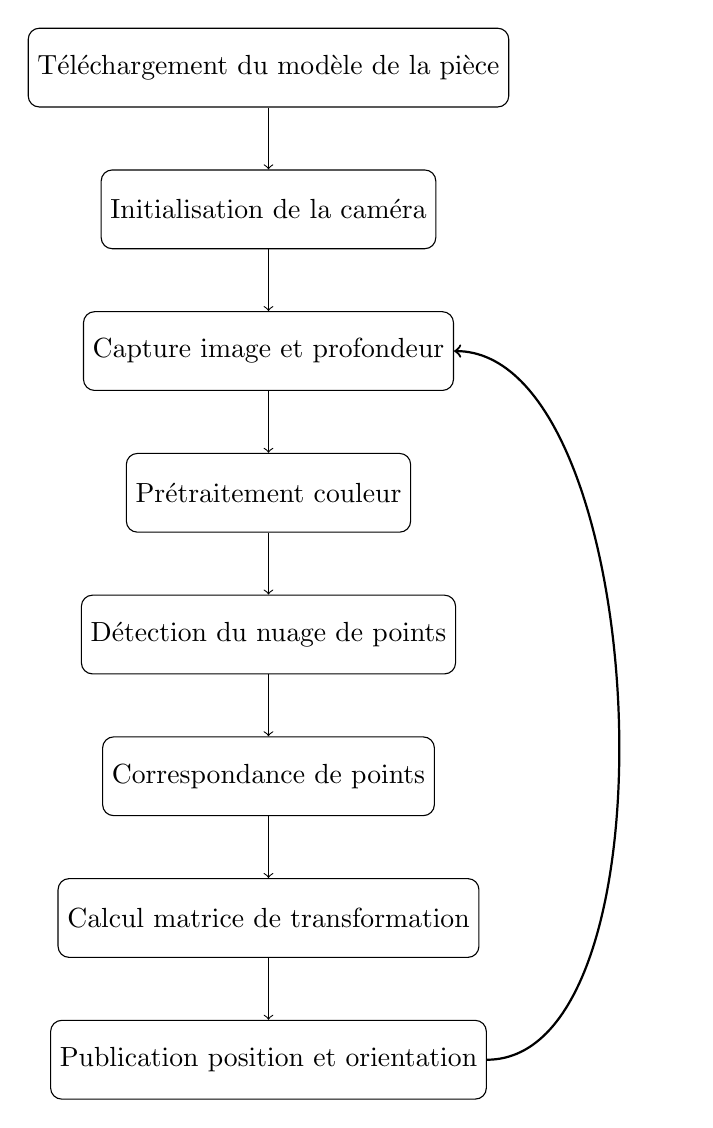
\begin{tikzpicture}[node distance=1.8cm, every node/.style={draw, align=center, rounded corners, minimum height=1cm}]

            \node (load) {Téléchargement du modèle de la pièce};
            \node (init) [below of=load] {Initialisation de la caméra};
            \node (capture) [below of=init] {Capture image et profondeur};
            \node (preprocess) [below of=capture] {Prétraitement couleur};
            \node (cloud) [below of=preprocess] {Détection du nuage de points};
            \node (match) [below of=cloud] {Correspondance de points};
            \node (matrice) [below of=match] {Calcul matrice de transformation};
            \node (publish) [below of=matrice] {Publication position et orientation};
            \draw[->] (load) -- (init);
            \draw[->] (init) -- (capture);
            \draw[->] (capture) -- (preprocess);
            \draw[->] (preprocess) -- (cloud);
            \draw[->] (cloud) -- (match);
            \draw[->] (match) -- (matrice);
            \draw[->] (matrice) -- (publish);
            \draw[->, thick] (publish.east) .. controls +(right:2.5cm) and +(right:2.5cm) .. (capture.east);
        \end{tikzpicture}
    \end{minipage}%
    \hfill
    \begin{minipage}{0.4\textwidth}
        \centering
        \begin{subfigure}{0.8\linewidth}
            \fbox{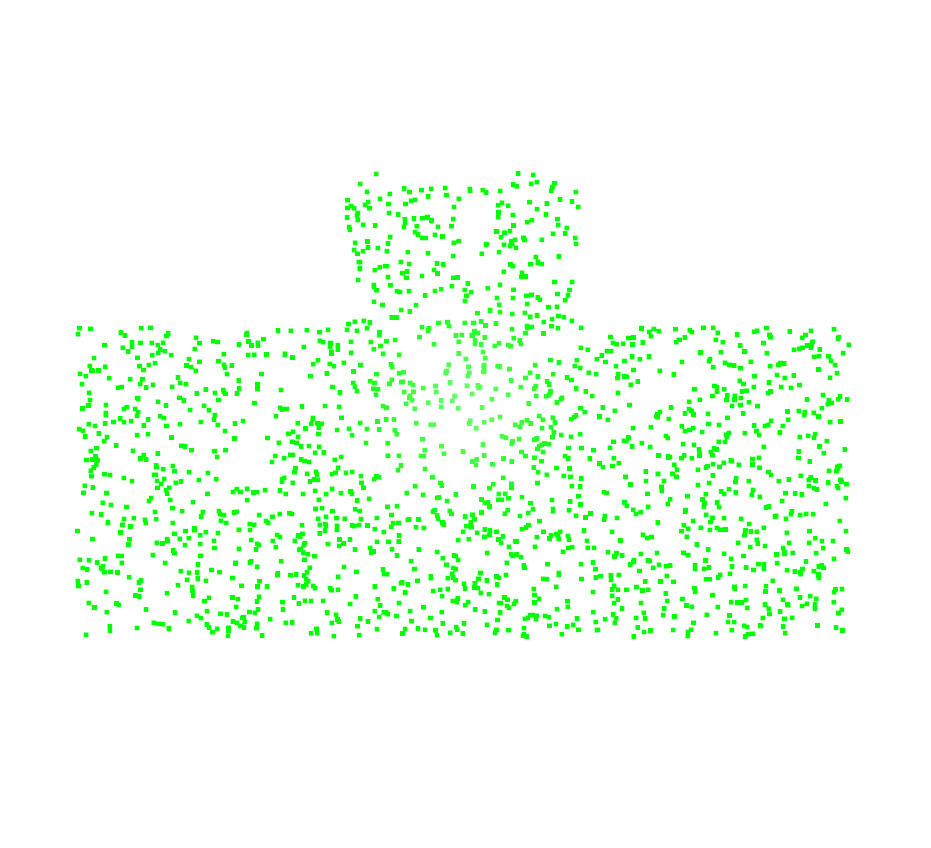
\includegraphics[width=\linewidth]{assets/figures/Piece_model.png}}
            \caption{Modèle 3D de la pièce}
        \end{subfigure}\\[0.2cm]
        \begin{subfigure}{0.8\linewidth}
            \fbox{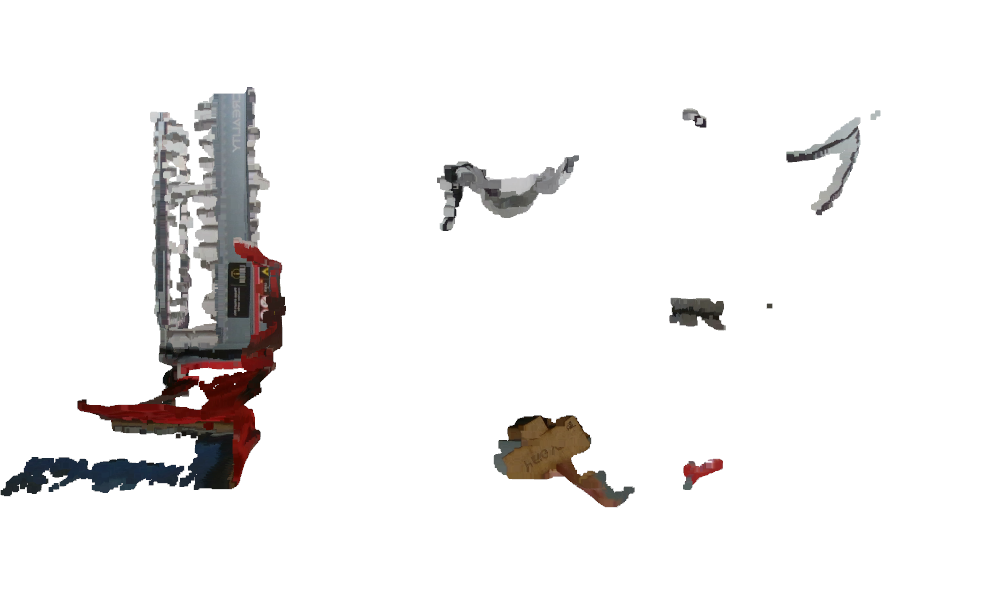
\includegraphics[width=\linewidth]{assets/figures/photo_origin.png}}
            \caption{Prise de la photo}
        \end{subfigure}\\[0.2cm]
        \begin{subfigure}{0.8\linewidth}
            \fbox{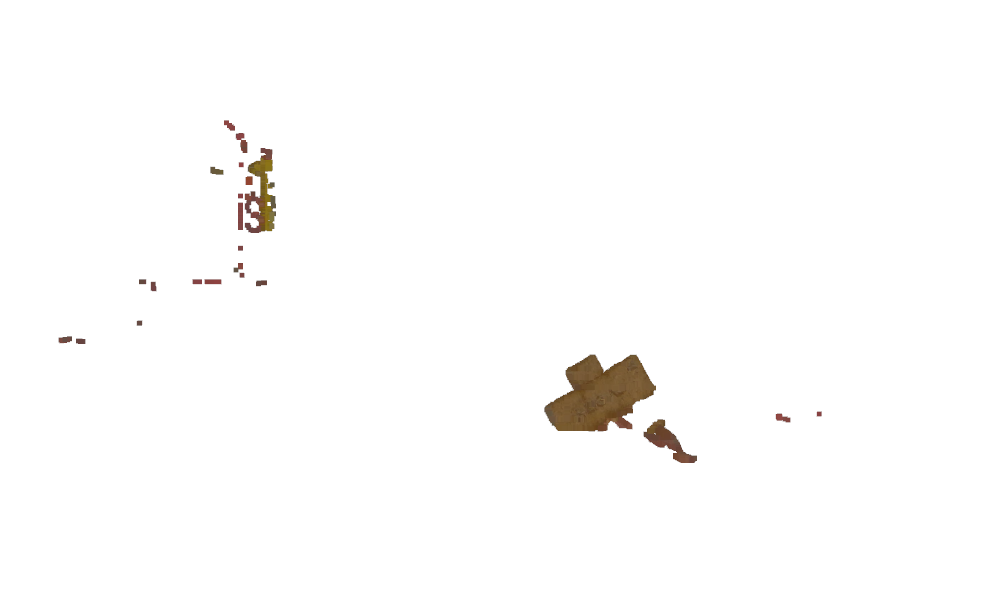
\includegraphics[width=\linewidth]{assets/figures/filtrage_couleur.png}}
            \caption{Filtrage par couleur}
        \end{subfigure}\\[0.2cm]
        \begin{subfigure}{0.8\linewidth}
            \fbox{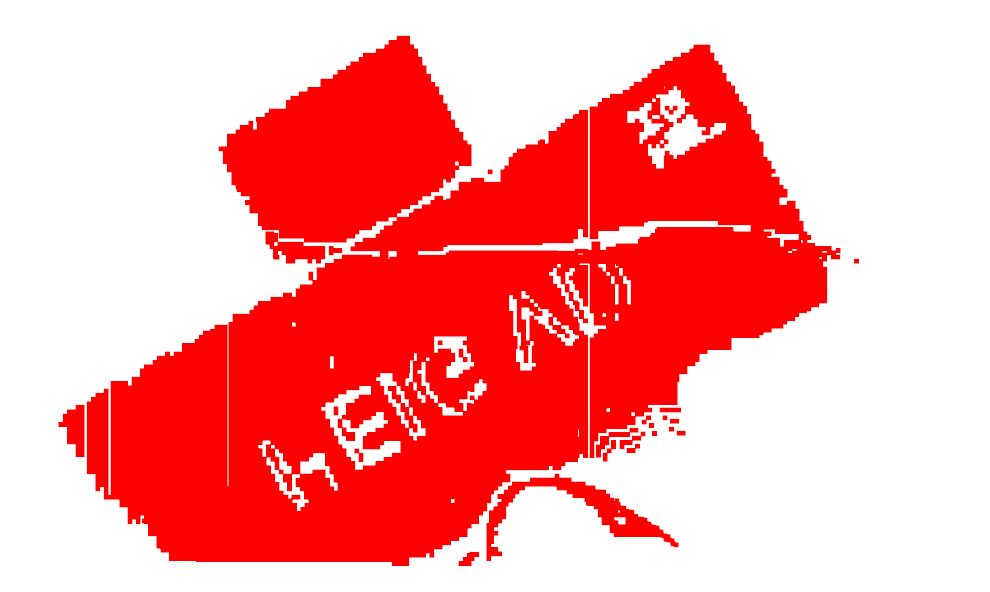
\includegraphics[width=\linewidth]{assets/figures/detection_piece.png}}
            \caption{Isolement de la pièce}
        \end{subfigure}\\[0.2cm]
        \begin{subfigure}{0.8\linewidth}
            \fbox{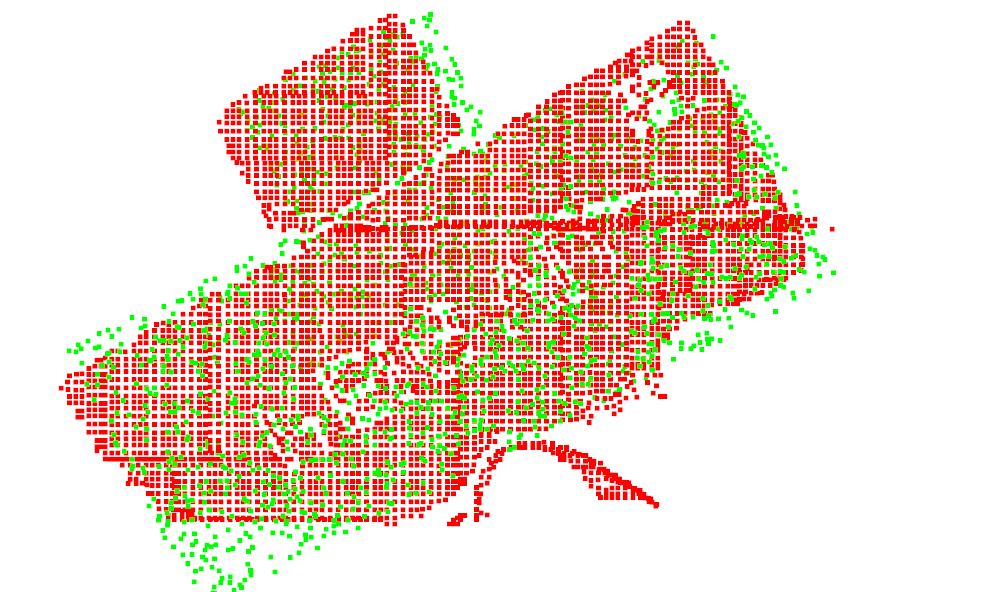
\includegraphics[width=\linewidth]{assets/figures/superposition.png}}
            \caption{Superposition modèle/réalité}
        \end{subfigure}
    \end{minipage}
    \caption{Schéma de séquence du programme de la caméra Intel D435, avec illustrations des étapes principales}
    \label{fig:sequence_camera_illustre}
\end{figure}

Tout comme le bloc fonctionnel de la graveuse laser, le bloc fonctionnel de la caméra offre une certaine liberté dans les paramètres de traitement. Il est par exemple possible de choisir la couleur de la pièce à détecter, modifier le modèle ainsi que le nombre de points de ce dernier. Cette flexibilité permet d'adapter le système tant dans la pièce à détecter que dans la rapidité de traitement. D'autres réglages sont aussi disponibles.

\begin{figure}[H]
    \centering
    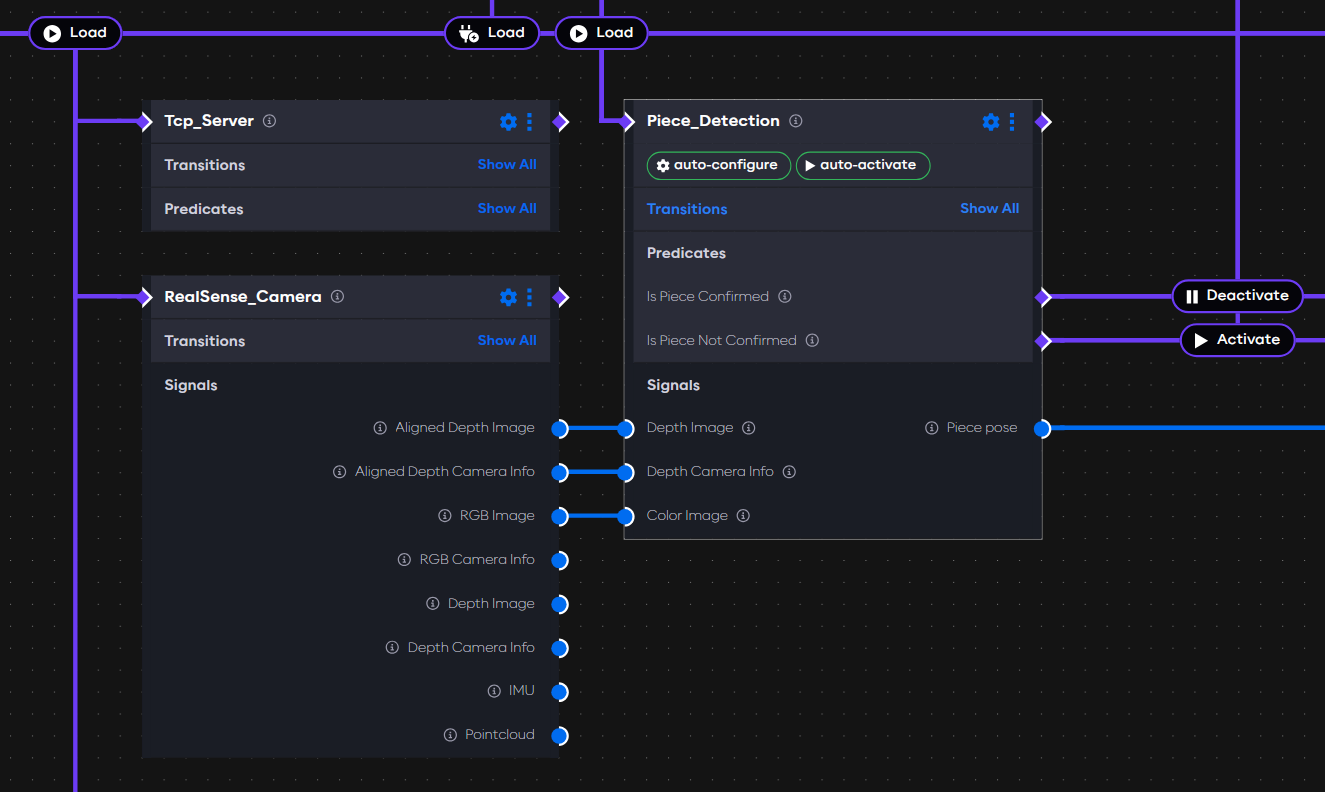
\includegraphics[width=0.8\textwidth]{assets/figures/AICA_Camera.png}
    \caption{Bloc fonctionnel de la caméra dans AICA Studio}
    \label{fig:camera_interface}
\end{figure}

\subsection{Transformation du repère caméra au repère robot}

Pour obtenir la position de la pièce détectée dans le repère du robot (ou du monde), le programme effectue une composition de transformations :

\begin{enumerate}
    \item \textbf{Détection de la pièce dans le repère caméra} :
          \begin{itemize}
              \item La position de la pièce est estimée en superposant le centroïde du modèle 3D (référence) et celui de la pièce détectée dans l'image. Cette position est donc exprimée dans le repère de la caméra.
              \item La rotation de la pièce est déterminée en testant différentes orientations (rotation degré par degré autour de chaque axe) et en cherchant celle qui aligne au mieux le modèle 3D avec la pièce détectée. Cette rotation est également exprimée dans le repère de la caméra.

              \inputminted[firstline=176, lastline=181, fontsize=\small, linenos, frame=lines, breaklines, bgcolor=gray!10]{python}{assets/code/piece_detection.py}
              \captionof{listing}{Rotation sur chaque axe pour trouver la meilleure orientation de la pièce dans le code python}
              \label{lst:piece_detection}

          \end{itemize}
    \item \textbf{Transformation du repère caméra au repère monde (robot)} :
          \begin{itemize}
              \item La position et l'orientation de la caméra dans le repère monde (ou robot) sont connues et définies par une translation et un quaternion (paramètre \texttt{camera\_pose\_world}).
              \item On construit la matrice de transformation homogène de la caméra dans le monde : $T_{\text{cam} \to \text{world}}$.
          \end{itemize}
    \item \textbf{Calcul de la position finale de la pièce dans le monde} :
          \begin{itemize}
              \item On compose la transformation de la pièce dans la caméra ($T_{\text{piece} \to \text{cam}}$) avec celle de la caméra dans le monde ($T_{\text{cam} \to \text{world}}$) :
                    \[
                        T_{\text{piece} \to \text{world}} = T_{\text{cam} \to \text{world}} \cdot T_{\text{piece} \to \text{cam}}
                    \]
              \item On obtient ainsi la position et l'orientation de la pièce dans le repère monde (robot), ce qui permet au robot de s'y rendre précisément.
          \end{itemize}
    \item \textbf{Implémentation dans le code} :
          \begin{itemize}
              \item Le code utilise la librairie \texttt{scipy.spatial.transform.Rotation} pour convertir les quaternions en matrices de rotation, et \texttt{numpy} pour manipuler les matrices de transformation.
          \end{itemize}
\end{enumerate}



Cette méthode permet de publier la position et l'orientation de la pièce dans le repère global, ce qui est indispensable pour que le robot puisse saisir ou interagir avec la pièce détectée.

\subsection{Valeurs de la matrice de transformation}

Dans ce projet, il n'a pas été nécessaire de réaliser une calibration manuelle entre la caméra et le repère robot. En effet, grâce au modèle 3D précis de la maquette, la position et l'orientation de la caméra ont pu être déterminées virtuellement, ce qui a permis de renseigner directement la matrice de transformation dans le programme.

\begin{minipage}{0.55\textwidth}
    \paragraph{Transformation caméra → monde}
    La pose de la caméra dans le monde utilisée dans le code est la suivante :
    \begin{itemize}
        \item Translation (m) : $[0.420451,\ 0.0175,\ 0.766251]$
        \item Quaternion (w, x, y, z) : $[0,\ -0.707107,\ 0.707107,\ 0]$
    \end{itemize}
    {\rowcolors{2}{}{}}%
    La matrice de transformation homogène correspondante est :
    \begin{equation*}
        T_{\text{cam} \to \text{world}} =
        \begin{bmatrix}
            0  & -1 & 0  & 0.420451 \\
            -1 & 0  & 0  & 0.0175   \\
            0  & 0  & -1 & 0.766251 \\
            0  & 0  & 0  & 1
        \end{bmatrix}
    \end{equation*}
    Cette transformation permet de passer des coordonnées caméra aux coordonnées monde (robot), ce qui est indispensable pour la localisation de la pièce par le robot.
\end{minipage}%
\hfill
\begin{minipage}{0.4\textwidth}
    \centering
    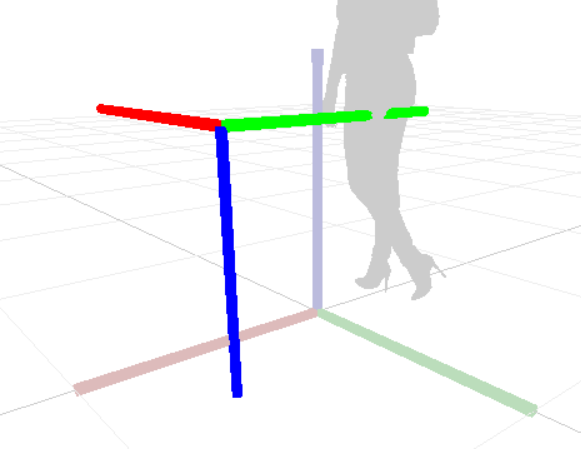
\includegraphics[width=0.95\linewidth]{assets/figures/Transform_example.png}
    \captionof{figure}{Illustration de la transformation de repère caméra vers monde}
\end{minipage}

\section{Programme AICA Studio}
Afin de faire fonctionner les différents blocs fonctionnels développés, il est donc nécessaire de les intégrer dans AICA Studio. A l'aide de blocs de base du logiciel et de certains blocs fournis après coup par l'entreprise, il a été possible de créer un programme qui relie tous les éléments de la maquette ensemble.
\begin{figure}[H]
    \centering
    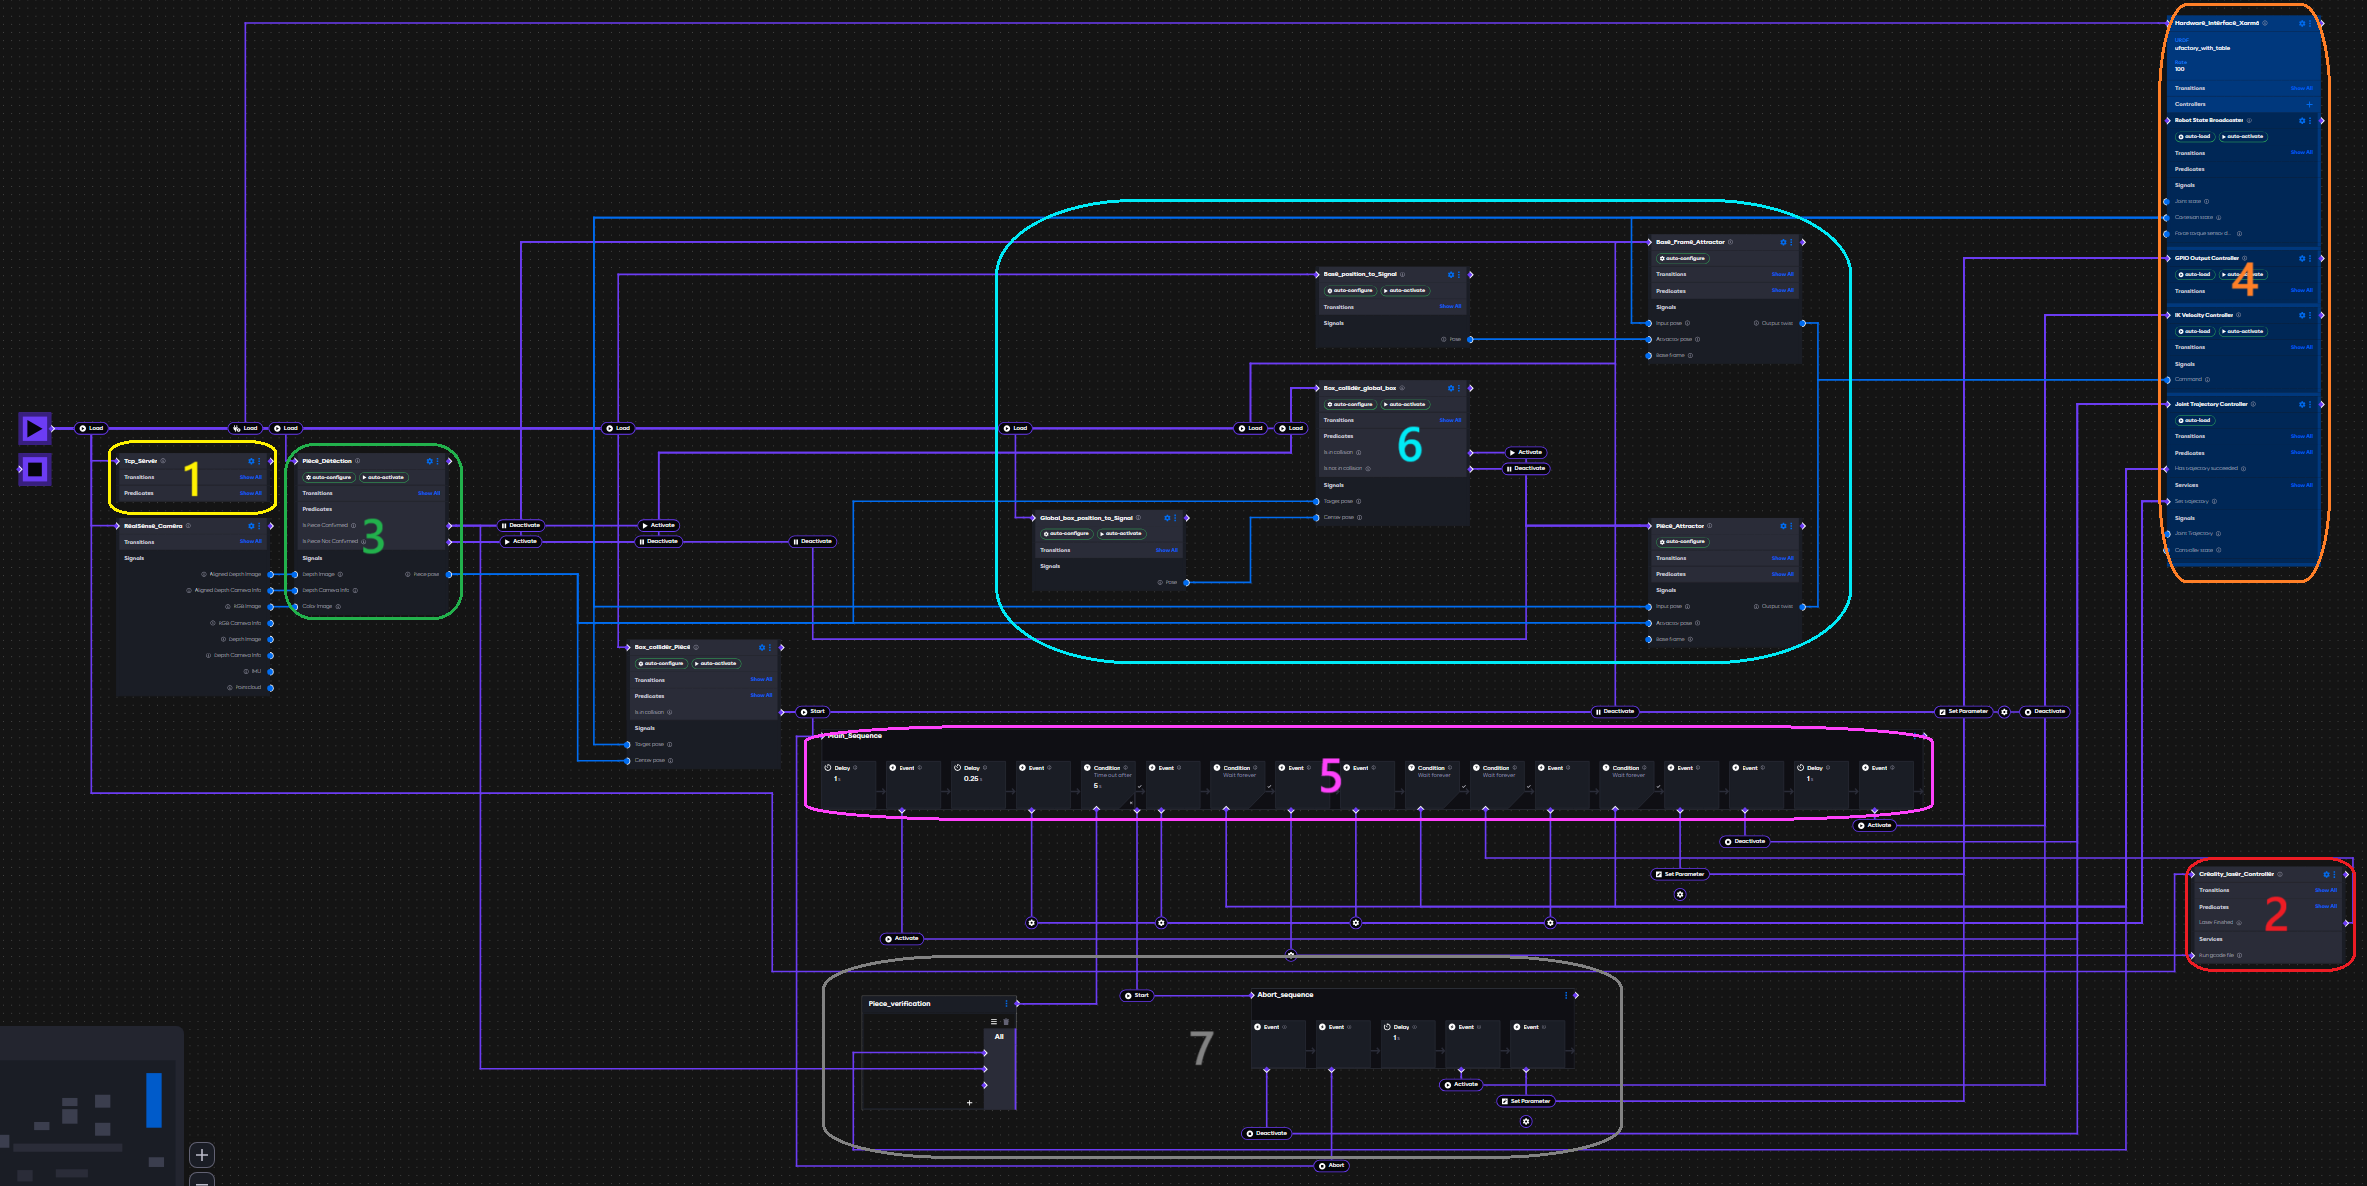
\includegraphics[width=0.8\textwidth]{assets/figures/AICA_PROG.png}
    \caption{Programme AICA Studio de la maquette de la graveuse laser intelligente}
    \label{fig:aica_programme}
\end{figure}

On constate beaucoup d'éléments différents dans le programme, notamment :
\begin{itemize}
    \item Le bloc TCP de communication avec le PC de l'écran tactile.
    \item Le bloc de la graveuse laser qui permet de charger le fichier DXF et de lancer la machine
    \item Le bloc de la caméra qui permet de détecter la position de la pièce.
    \item Le bloc du bras robot qui permet de communiquer directement avec l'appareil
    \item Le bloc de séquence qui permet de gérer l'ordre d'exécution des différentes tâches lorsque le robot attrape une pièce.
    \item Les blocs de gestion de prise de pièce qui assurent une approche correcte et une préhension efficace.
    \item Les blocs de gestion de vérification de prise de pièce et d'avortement de la tâche en cours si nécessaire.
\end{itemize}

Certains de ces blocs ou groupes de blocs on déjà étés expliqués ci-dessus, d'autres serons détaillés dans les sections suivantes.

\subsection{Bloc du bras robot}

Le bloc du bras robot est ce qui permet la communication entre le programme et les différents actionneurs du robot. Avec plusieurs options de contrôleurs, il est possible de piloter le robot de plusieurs manières différentes (mais pas en même temps). Dans le cas de la maquette, ce sont un contrôle de vélocité et un contrôle de trajectoire qui sont utilisés. Le bloc permet également de gérer l'ouverture et la fermeture de la pince.

\begin{figure}[H]
    \centering
    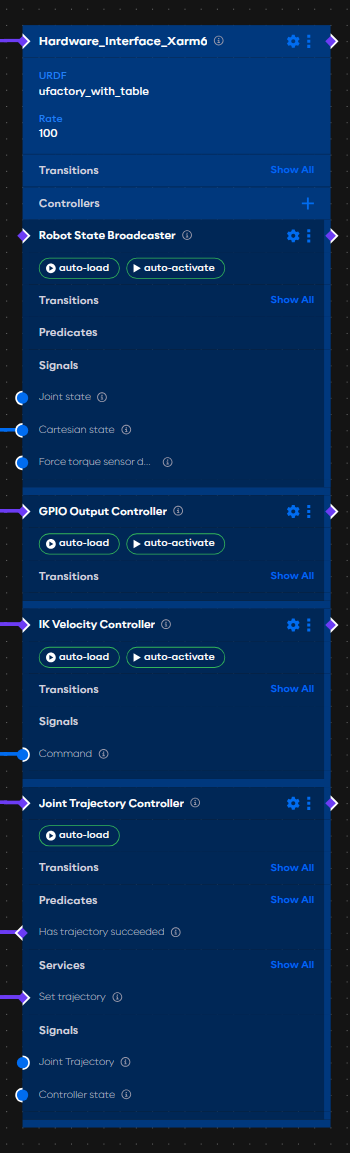
\includegraphics[width=0.8\textwidth]{assets/figures/AICA_Hardware_interface.png}
    \caption{Bloc du bras robot dans AICA Studio}
    \label{fig:robot_block}
\end{figure}

On constate plusieurs entrées et sorties dans le bloc du bras robot qui se réunissent en trois types :
\begin{itemize}
    \item L'entrée d'activation ou de désactivation du bloc entiers.
    \item Les entrées de commande du robot.
    \item Les sorties d'états du robot.
\end{itemize}


Dans le cas des sorties d'états du robot, toutes ne sont pas utilisées dans ce projets et donc n'apparaissent pas sur l'illustration.

\subsection{Bloc de séquence}

Le bloc de séquence est utilisé dans la seconde partie du programme. Il sert à traiter des événements tel que des déplacements ainsi que l'envoi et la réceptiond de signaux.

\begin{figure}[H]
    \centering
    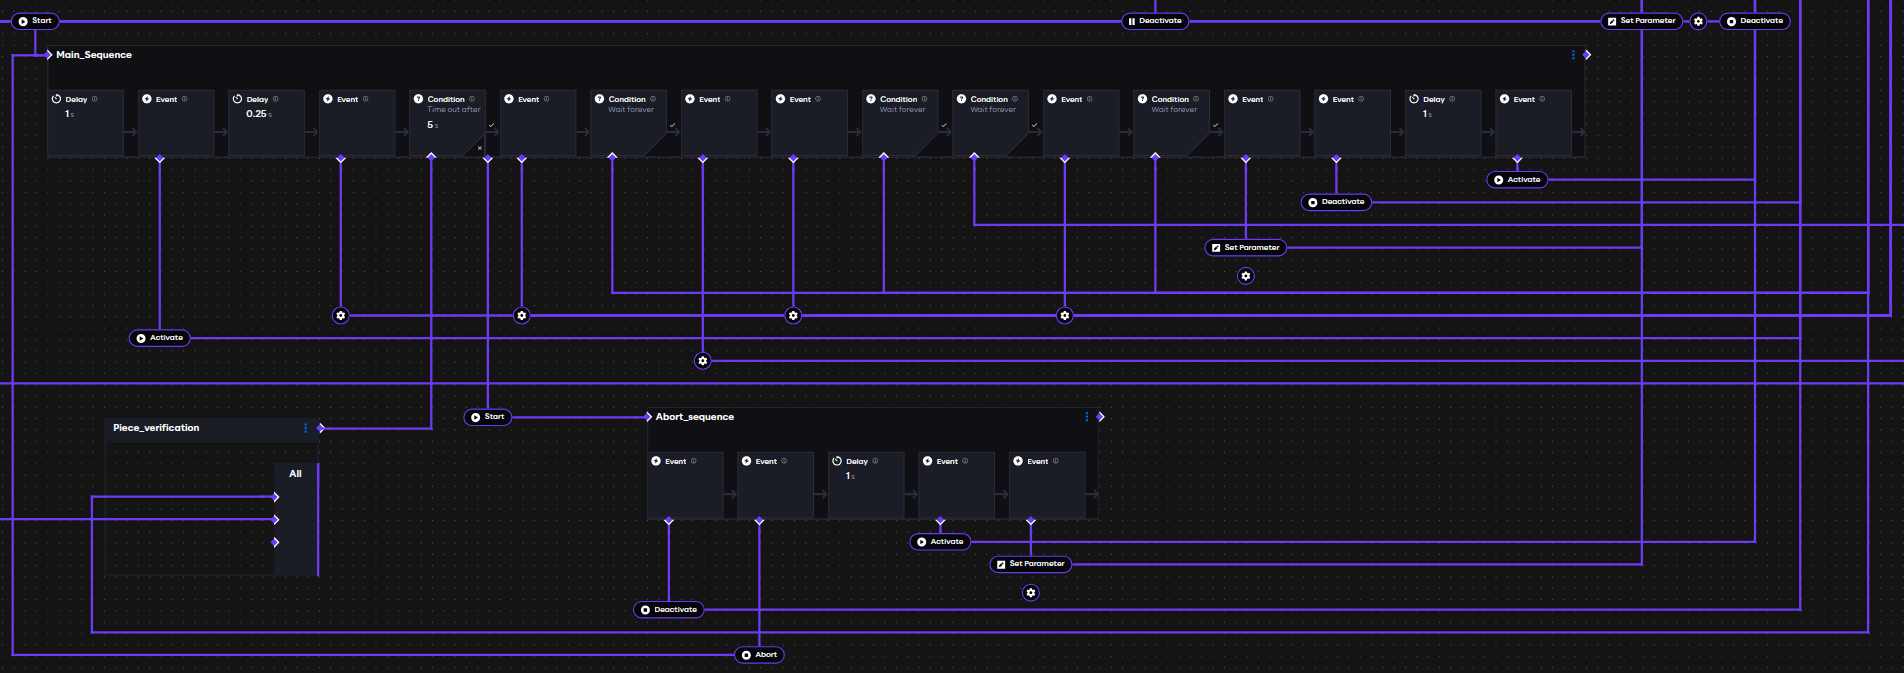
\includegraphics[width=0.8\textwidth]{assets/figures/AICA_Sequence (2).png}
    \caption{Bloc de séquence dans AICA Studio}
    \label{fig:sequence_block}
\end{figure}

(partie à modifier) Dans ce cas, le bloc de séquence est activé après que le robot ait saisi la pièce. Dans un premier temps, un délai d'une seconde est appliqué pour laisser le temps à l'un des contrôleur du robot de se désactiver. ensuite le signal est donné au second contrôleur de s'activer et un second délais est laissé. Ensuite, pour faciliter la compréhension du programme, toutes les connexions qui vont au même endroit sont sur la même ligne. On peut donc voir que le quatrième élément de la séquence est une commande de position. D'autres commandes de positions sont alors identifiables en septième et dixième position. Le cinquième élément lui, est un signal venant du robot qui ne s'active que quand le robot à fini de se déplacer. Cela permet de contrôler le déroulement de la séquence en mettant des points de vérifications dans le cas ou un mouvement ne se passe pas comme prévu. Les éléments 8 et 11 sont aussi des retours. Le sixième élément est un signal qui va directement dans le bloc d'interface avec la graveuse laser. C'est lui qui s'occupe de démarrer la graveuse laser. L'élément 9 est un signal de retour venant du bloc d'interface de la graveuse laser. Il est utilisé pour savoir si la graveuse a fini de graver ou non. Ensuite le douzième élément est un signal envoyé au bloc robot pour ouvrir la pince. Pour terminer, les trois derniers éléments remettent le programme dans sa position de départ, en désactivant le contrôleur utilisé par la séquence et en réactivant le contrôleur utilisé pour la prise de la pièce. (partie à modifier)

\subsection{Blocs de gestion de prise de pièce}

Les blocs de gestion de prise de la pièce sont divisées en deux parties qui fonctionnent en alternance. La première partie est utilisée pour l'approche de la pièce et la seconde pour le retour dans la position de départ dans le cas ou la pièce n'est plus détectée. L'avantage de cette approche est que le robot se met automatiquement dans la position de départ au démarrage du programme.

\begin{figure}[H]
    \centering
    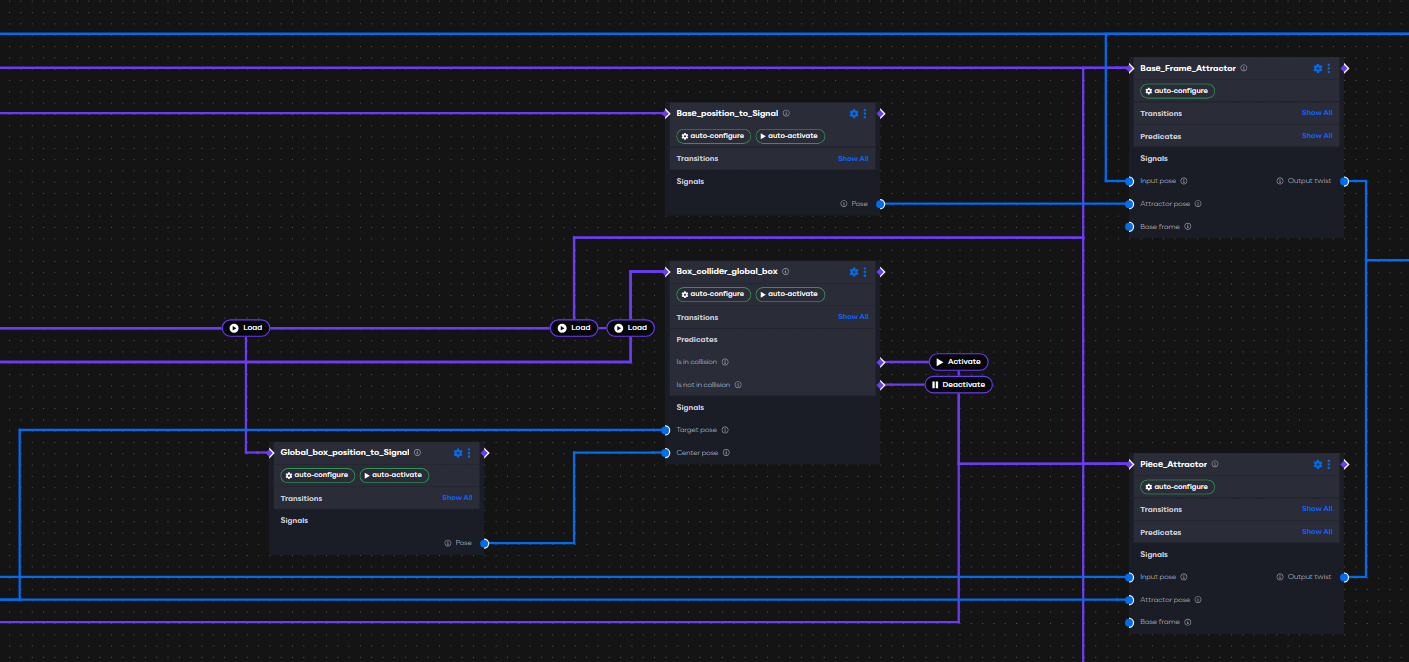
\includegraphics[width=0.8\textwidth]{assets/figures/AICA_Prise (2).png}
    \caption{Blocs de gestion de prise de pièce dans AICA Studio}
    \label{fig:piece_block}
\end{figure}


Le fonctionnement de ces blocs repose sur une logique d'alternance entre deux états principaux : l'approche de la pièce et le retour à la position de départ. Lorsqu'une pièce est détectée par la caméra, le robot reçoit la position cible et commence à s'approcher de la pièce en suivant la trajectoire calculée. Si, à tout moment, la pièce n'est plus détectée (par exemple, si elle a été retirée), le robot interrompt son mouvement et retourne automatiquement à sa position de départ pour attendre une nouvelle détection.

Cette logique permet d'assurer la sécurité et la robustesse du système: le robot ne tente jamais de saisir une pièce absente et se remet toujours dans une position sûre en cas d'erreur ou d'absence de détection. De plus, cela facilite la reprise du processus dès qu'une nouvelle pièce est détectée, sans intervention manuelle.

L'implémentation de cette alternance est réalisée à l'aide du bloc de détection de la pièce, qui envoie active ou désactive les blocs en fonction de si la pièce est détectée ou non.


\subsection{Blocs de vérification et d'avortement}

Les blocs de verification et d'avortement sont des éléments de sécurité ajoutés afin de s'assurer que le robot ne continue pas sa séquence si la pièce n'est pas prise. Cela rajoute un point de sécurité qui minimise donc les conséquences d'une mauvaise prise de la pièce.  Cette décision à été prise suite a l'élaboration du tableau des risques du \textbf{chapitre \ref{chap:analyse}}.

\begin{figure}[H]
    \centering
    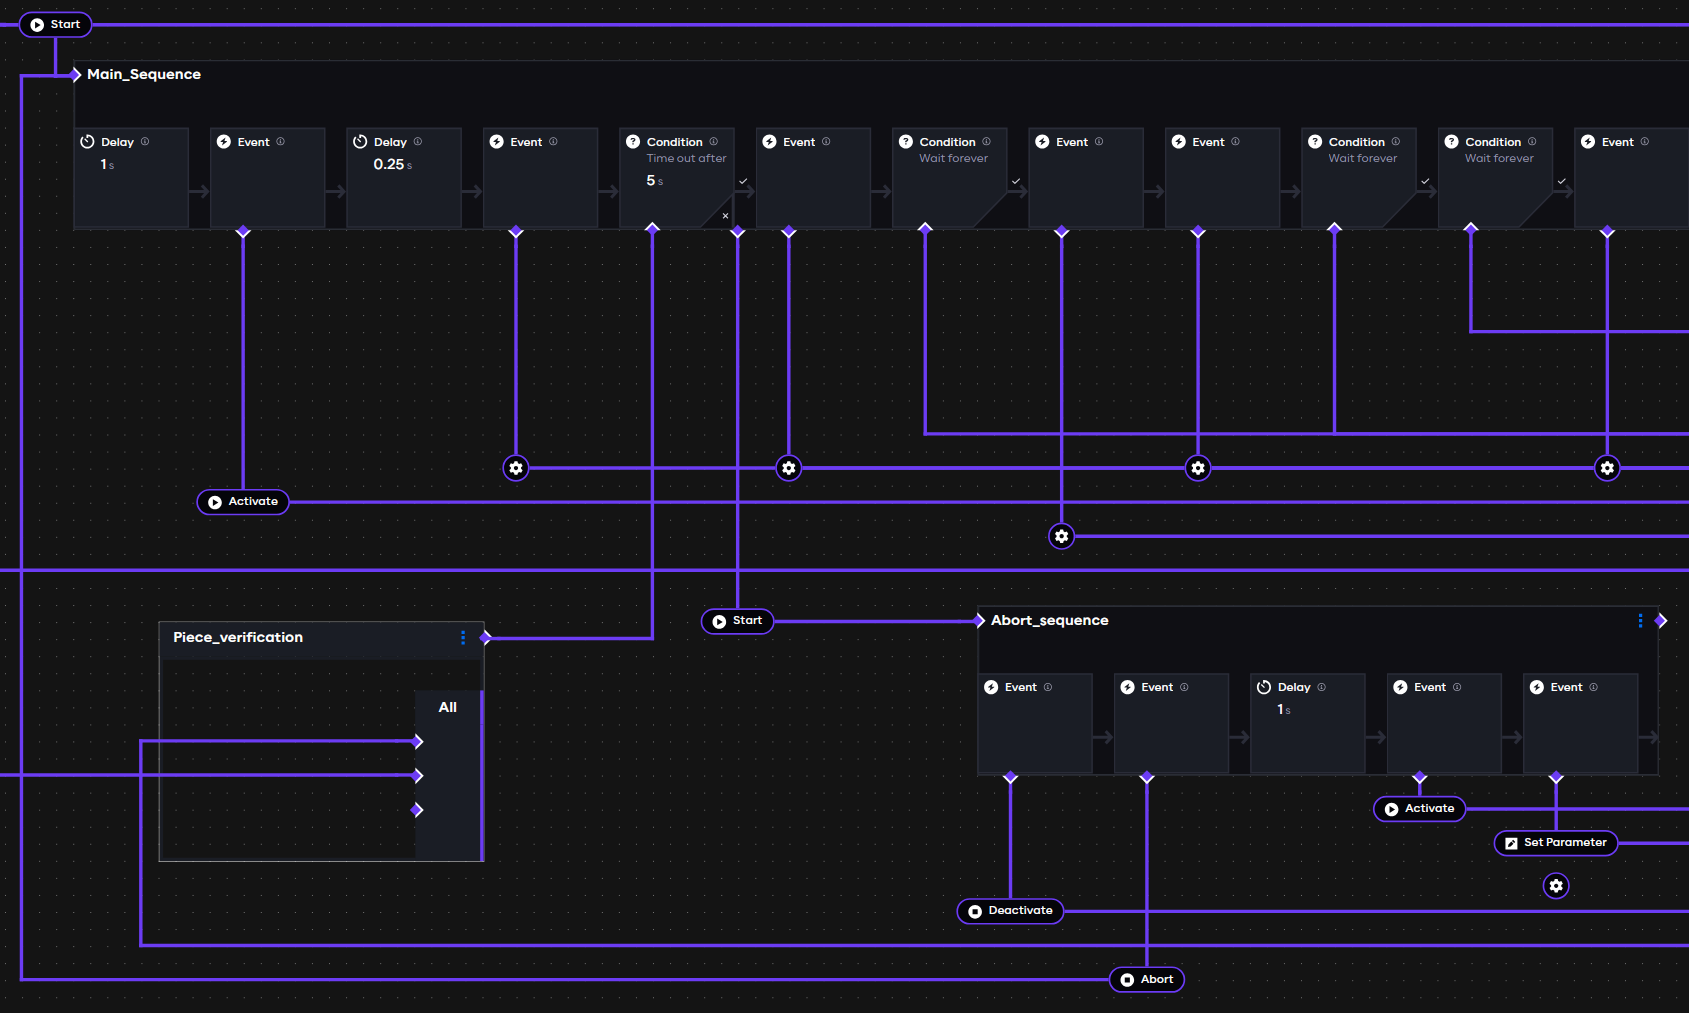
\includegraphics[width=0.8\textwidth]{assets/figures/AICA_Abort_sequence.png}
    \caption{Blocs de vérification et d'avortement dans AICA Studio}
    \label{fig:verification_block}
\end{figure}

On peut voir une intéraction directe entre le bloc de séquence principale et le bloc d'avortement. Cela est du à la nécessité d'arreter la séquence principale si jamais la pièce n'est pas dans les pinces du robot au moment de la vérification. En amont, un bloc logique \textbf{ET} permet de prendre le signal de détection de pièce et le signal de validation de position venant du bloc du robot pour faire la vérification. Le robot reste attends la validation pendant 5 secondes. Si la validation n'est pas faite, le robot retourne en position de départ et la séquence est avortée. Si la validation est faite, le robot continue sa séquence normalement.

\subsection{Programmation des mouvements}

Afin de pouvoir faire bouger le robot dans le bloc de séquence, il est nécessaire d'envoyer un \gls{payload} au robot. Ce bout de code est ensuite déchiffré par le bloc du robot et traduis en mouvements.

\begin{figure}[H]
    \centering
    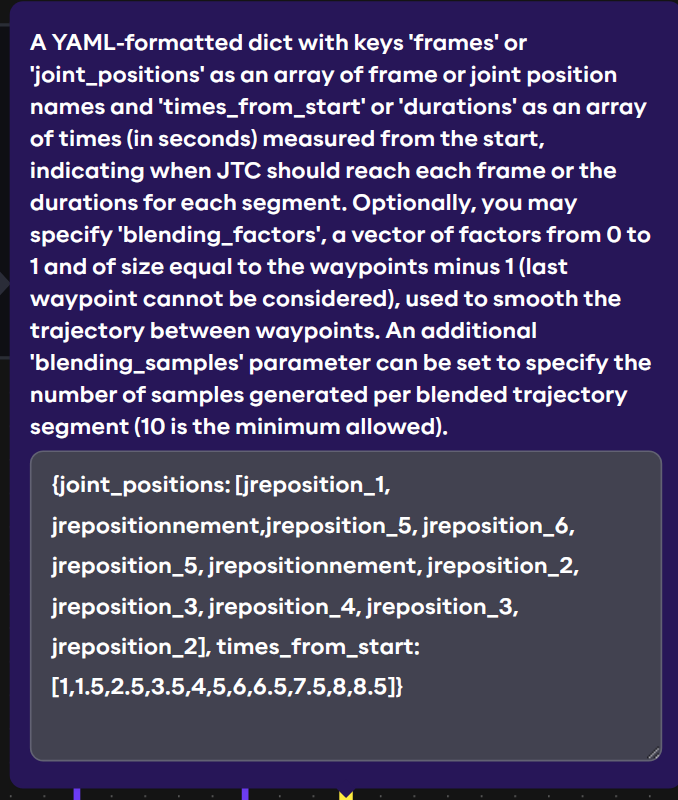
\includegraphics[width=0.8\textwidth]{assets/figures/AICA_payload.png}
    \caption{Bloc de programmation des mouvements dans AICA Studio}
    \label{fig:payload_block}
\end{figure}

Dans ce cas, la liste des mouvements est données en premier sous forme de positions articulaires. Ensuite, les chiffres correspondent au moment ou chaque position doit être atteinte. Cette approche permet de contrôler précisément le temps total de la séquence mais rend toute modification compliquée. En effet, si l'on souhaite modifier la durée d'un mouvement, il faut recalculer tous les mouvements suivants pour que le robot arrive à la bonne position au bon moment. Cela peut être un inconvénient si l'on souhaite faire des modifications fréquentes ou pendant la phase de test. Néanmoins, dans une mise à jour récente, la possibilité de modifier la durée de chaque mouvement indépendament des autres a été ajoutée.

Il est aussi possible de donner des points dans l'espace avec une orientation plutôt qu'une configuration articulaire fixe. Cette possibilité est plus simple à mettre en place mais est utile pour des positions et mouvements moins exigeants que ceux programmés dans le projet. Le bras robot possédant deux axes pouvants tourner à plus que 360 degrés, il se retrouvais régulièrement dans des situations ou les axes étaients proche des limites de leur rotation. Cela rendait le robot imprévisible et menais à des erreurs aléatoires qui bloquaient le système.
